\documentclass[aspectratio=169]{beamer}

\usepackage{graphicx}
\usepackage{hyperref}
\usepackage{amstex}

\title{Clever Party Thrower}

\author{Louis De Wilde}
\date{\today}

\begin{document}

    \frame{\titlepage}
    \begin{frame}
        \frametitle{Un peu de contexte}
        Quel est le problème ?
        \begin{itemize}
            \item Facilité le choix d'une date
            \item Répartir le coût d'un événement entre les participants
            \item Toutes les informations sur un événement au même endroit
            \item L'application peut être déployée on-premise
        \end{itemize}
        Qui a ce problème ?
        \begin{itemize}
            \item Des particuliers qui souhaitent organiser des événements
            \item Des petits organisateurs d'événements par exemple un cercle étudiant
        \end{itemize}
    \end{frame}


    \begin{frame}
        \frametitle{Pourquoi utiliser Clever Party Thrower et pas d'autres applications ?}
        \begin{columns}
            \begin{column}{0.5\textwidth}
                \begin{itemize}
                    \item Tout au même endroit
                    \item Respectueux de la vie privée
                    \item Open Source
                    \item Simple d'accès
                    \item Gratuit
                \end{itemize}
            \end{column}

            \begin{column}{0.3\textwidth}
                \begin{flushleft}
                    
\includegraphics[width=1\textwidth]{imgs/selfHost&opensource}\label{fig:figure8}
                \end{flushleft}
            \end{column}
            \begin{column}{0.2\textwidth}

            \end{column}
        \end{columns}

    \end{frame}

    \begin{frame}
        \frametitle{Technologies utilisées \& Analyse}
        \begin{figure}[h]
            \centering
%            
\includegraphics[width=0.15\textwidth]{imgs/Angular}
%            
\includegraphics[width=0.1\textwidth]{imgs/Ansible}
%            
\includegraphics[width=0.15\textwidth]{imgs/Docker}
%            
\includegraphics[width=0.15\textwidth]{imgs/Kube}
%            
\includegraphics[width=0.1\textwidth]{imgs/cermanager}
%            
\includegraphics[width=0.1\textwidth]{imgs/apollo}
%            
\includegraphics[width=0.1\textwidth]{imgs/argo}
%            
\includegraphics[width=0.1\textwidth]{imgs/Cloudflare}
%            
\includegraphics[width=0.1\textwidth]{imgs/watchtower}
%            
\includegraphics[width=0.1\textwidth]{imgs/Typescript}
%            
\includegraphics[width=0.1\textwidth]{imgs/TypeOrm}
%            
\includegraphics[width=0.1\textwidth]{imgs/Traefik}
%            
\includegraphics[width=0.1\textwidth]{imgs/totp}
%            
\includegraphics[width=0.1\textwidth]{imgs/SCSS}
%            
\includegraphics[width=0.1\textwidth]{imgs/rxjs}
%            
\includegraphics[width=0.1\textwidth]{imgs/rancher}
%            
\includegraphics[width=0.1\textwidth]{imgs/proxmox}
%            
\includegraphics[width=0.1\textwidth]{imgs/prisma}
%            
\includegraphics[width=0.1\textwidth]{imgs/Postgres.svg}
%            
\includegraphics[width=0.1\textwidth]{imgs/passport}
%            
\includegraphics[width=0.1\textwidth]{imgs/Openstreetmap}
%            
\includegraphics[width=0.1\textwidth]{imgs/nodejs}
%            
\includegraphics[width=0.1\textwidth]{imgs/nginx}
%            
\includegraphics[width=0.15\textwidth]{imgs/NestJS}
%            
\includegraphics[width=0.1\textwidth]{imgs/metalLb}
%            
\includegraphics[width=0.1\textwidth]{imgs/k3s}
%            
\includegraphics[width=0.1\textwidth]{imgs/longhorn}
%            
\includegraphics[width=0.1\textwidth]{imgs/letsencrypt}
%            
\includegraphics[width=0.1\textwidth]{imgs/kube-vip}
%            
\includegraphics[width=0.1\textwidth]{imgs/joi}
%            
\includegraphics[width=0.1\textwidth]{imgs/html}
%            
\includegraphics[width=0.1\textwidth]{imgs/helm}
%            
\includegraphics[width=0.1\textwidth]{imgs/gql}
%            
\includegraphics[width=0.1\textwidth]{imgs/github}
%            
\includegraphics[width=0.15\textwidth]{imgs/gitAction}
%            
\includegraphics[width=0.1\textwidth]{imgs/falso}
%            
\includegraphics[width=0.1\textwidth]{imgs/ESLint}
%            
\includegraphics[width=0.1\textwidth]{imgs/dicebear}
%            
\includegraphics[width=0.1\textwidth]{imgs/docker-compose}
            
\includegraphics[width=1\textwidth]{imgs/used tech}\label{fig:figure}
        \end{figure} %sur base des criteres j'ai decide que une web app cosrespondais , j'ai decider d'utiliser un maximum de technologie affin de rendre le projet robuste et facile a ameliorer/modifier
    \end{frame}



    \begin{frame}
        \frametitle{Développement de l'API}
%        Le backend est la partie qui a demandé le plus de travail
        \begin{columns}
            \begin{column}{0.5\textwidth}
                \begin{itemize}
                    \item Robuste Testing, Typage
                    \item Modulaire
                \end{itemize}
            \end{column}

            \begin{column}{0.5\textwidth}
                \begin{flushleft}
                    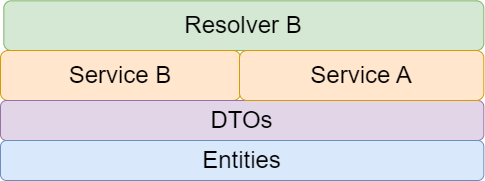
\includegraphics[width=0.7\textwidth]{imgs/module}\label{fig:figure4}
                \end{flushleft}
            \end{column}
        \end{columns}

    \end{frame}

    \begin{frame}%        Les concept d'integration, de deploiement et de gitops on ete implementer tout au long du projet
        \frametitle{Aspect DevOps}
        \begin{columns}
            \begin{column}{0.5\textwidth}
                \begin{itemize}
                    \item Intégration continue
                    \item Déploiement continu
                    \item GitOps
                    \item Conteneurisation
                    \item Infrastructure as Code
                    \item Hébergement
                    \subitem Docker-compose
                    \subitem Kubernetes
                \end{itemize}

            \end{column}
            \begin{column}{1\textwidth}
                \begin{flushleft}
                    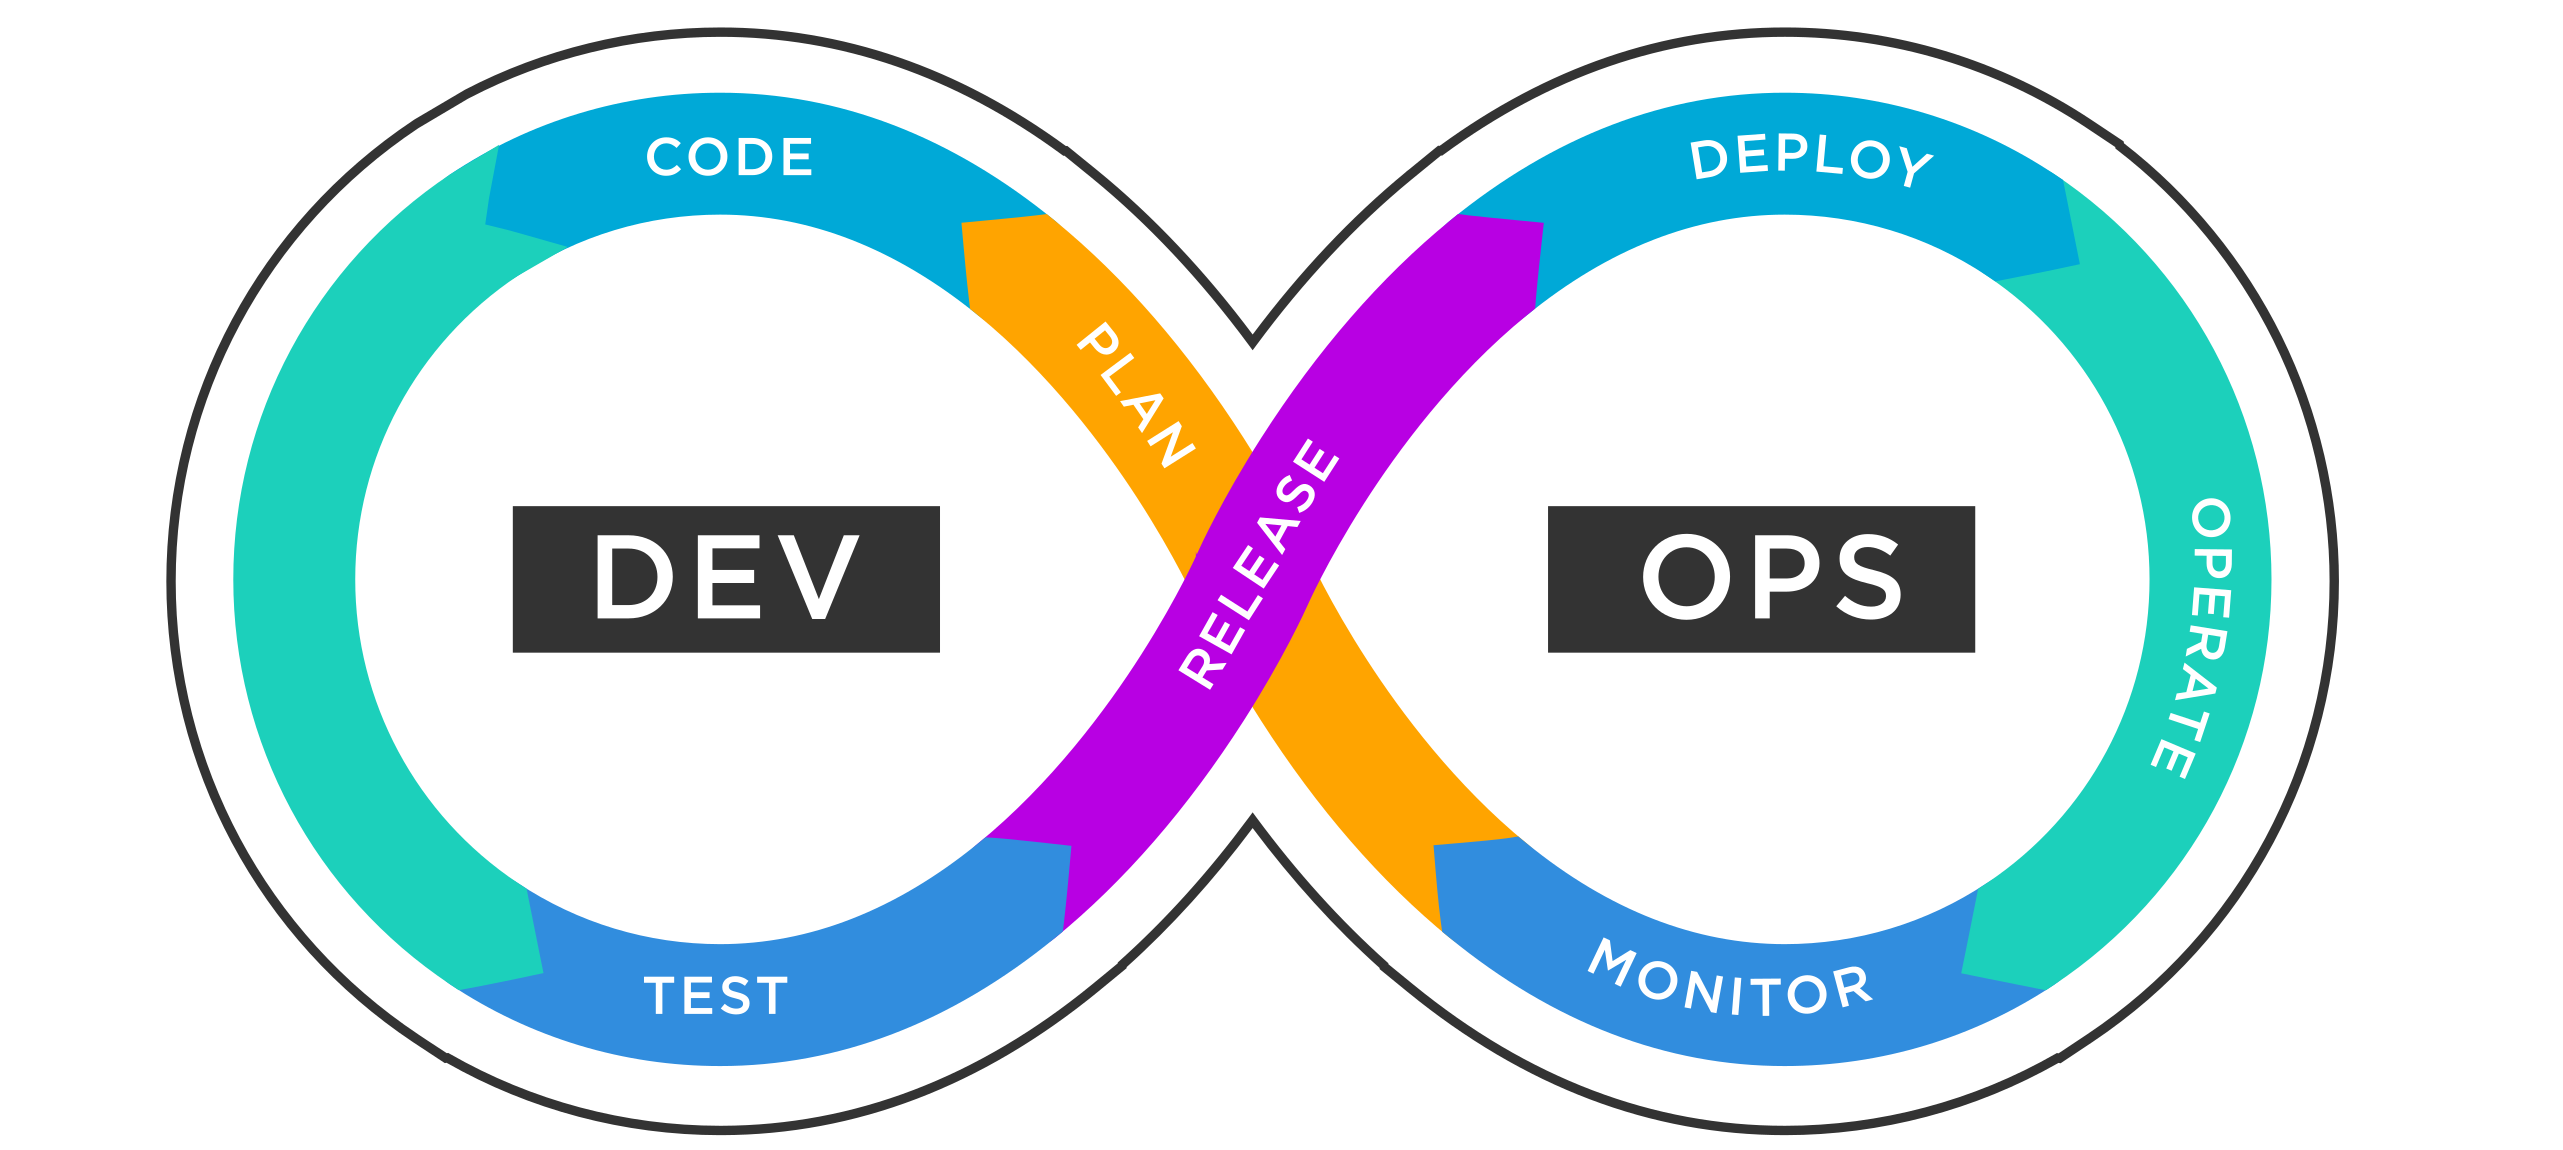
\includegraphics[width=0.50\textwidth]{imgs/devops}\label{fig:devops2}
                \end{flushleft}
            \end{column}
        \end{columns}
    \end{frame}

    \begin{frame}
        \frametitle{Interface utilisateur}
        \begin{columns}
            \begin{column}{0.5\textwidth}
                \begin{itemize}
                    \item Angular
                    \item RxJs
                    \item Apollo
                \end{itemize}
            \end{column}
            \begin{column}{0.5\textwidth}
                \begin{flushleft}
                    
\includegraphics[width=1\textwidth]{imgs/frontToBack}\label{fig:diagram}
                \end{flushleft}
            \end{column}
            \begin{column}{0.2\textwidth}

            \end{column}
        \end{columns}


    \end{frame}

    \begin{frame}
        \frametitle{Sécurité, vie privée et législation}
        \begin{itemize}
            \item Chiffrement et authentification
            \item Contremesures
            \subitem Injection SQL,
            \subitem SSL et HTTPS,
            \item RGPD
            \subitem Gestion des données
            \subitem Minimum de données
            \subitem Suppression des données
        \end{itemize}
        \begin{figure}[h]
            \centering
            
\includegraphics[width=0.4\textwidth]{imgs/young-hacker-cyber-securty-concept-260nw-1450697288}\label{fig:figure5}
        \end{figure}

    \end{frame}

    \begin{frame}
        \frametitle{Petite démo}
        L'application est disponible en ligne via le qrcode
        \begin{figure}[h]
            \centering
            
\includegraphics[width=0.4\textwidth]{imgs/QRcode_C2 (5)}\caption{https://cpt.louisdewilde.be}\label{fig:figure2}
        \end{figure}
    \end{frame}

    \begin{frame}
        \frametitle{Améliorations futures}
        \begin{itemize}
            \item Ajout de nouvelles fonctionnalités
            \item Amelioration de l'interface web
            \item Déploiement de l'application avec Kubernetes
            \item Creation d'une page d'accueil qui explique le concept de l'application
        \end{itemize}
    \end{frame}

    \begin{frame}
        \centering
        \frametitle{Place à vos questions}
        %todo: add illustration
        \begin{figure}[h]
            \centering
            
\includegraphics[width=0.4\textwidth]{imgs/question-mark-speech-bubble-isolated-260}\label{fig:figure3}
        \end{figure}
    \end{frame}

\end{document}